\TOWRITE{ALL}{Proofread 1.2 up to 1.2.10}

\TOWRITE{ALL}{Write missing sections 1.2.13 to 1.2.16}

\TOWRITE{Min/Hans}{Mention KPIs somewhere?}

\TODO{Provide contents for empty subsections at the end of section 1.}

\subsection{Methodology}\label{sec:concept_methodology}
\eucommentary{5-8 pages}





% \subsubsection{Concept}%\label{sec:concept}
%
% Open Science is the principle that science, in order to be most
% {impactful} and {socially responsible}, should be done
% {publicly}, with as much of the scientific process and products
% accessible, reviewable, reproducible and reusable by as many members of
% the global community as possible.
%
% There are exciting opportunities for Open Science for almost all academic fields
% in the modern age of computational science. As more and more research takes the
% form of code and/or data, the opportunity to share, reproduce, and reuse
% scientific work is greater than ever, even enabling new forms of
% {interdisciplinary collaboration}, and interoperable and reusable results and
% tools.
%
%  Simultaneously, there are obstacles -- both technical and social -- to
% making open science and reproducible science a practical reality. The challenges
% include: If a researcher has code and/or data to publish, how is that best
% done? How do researchers learn {best practices for reproducible science} in
% their field? How do previously disconnected fields benefit from each other's
% work as the same computational challenges are faced again and again by different
% communities? How can scientists be encouraged to make their work reproducible?
%
% These are the questions that guide the \TheProject{} project.

\paragraph*{Supporting Open, Useful, and Reproducible Computational
  Environments}\label{sec:SOURCE} 

  \mbox{}\\

  The ideas behind our project title:
\begin{itemize}
\item The work done is this project will be \textbf{Supporting} scientists in their
  endeavours to make their work more reproducible and reusable.
\item We believe in the value of \textbf{Open} science and \textbf{Open} source software.
  The best reproducibility and reusability of scientific results is given through
  complete transparency of the steps taken in the derivation of a result. For
  the computational aspects this means to make all simulation and/or
  post-processing and analysis steps open source. While this may not always be
  possible, we advocate such openness as the best practice for reproducible science.

  All work done, including software, training and documentation materials, will
  be open source and available through an open access license. (We note that the
  collective development of the grant proposal you are reading is also done as
  open source, and can be inspected at \url{http://github.com/minrk/horizon-widera-2022}.)

\item Measures towards better reproducibility have to be \textbf{Useful} and
  practical: if a proposed approach or tool burdens the scientist with
  additional work, or requires significant additional skills, it becomes less
  likely to be widely accepted.

  The philosophy we support here is that the proposed (Binder) tools for
  reproducibility are based on existing standards which are already
  adopted by many and can be considered best practice.

\item Within the wide field of reproducibility in science, we focus in this
  project on the improvement of the automatic generation of \textbf{Reproducible
    Computational Environments}.
  % It is an essential step for reproducible
  % science to be able to setup the correct
  % software environment, before any attempt can be undertaken to reproduce (and
  % thus repeat) the calculation of a result obtained before.
\end{itemize}

\subsubsection{Outline of concept and methodology}

In the following we explain our concept and the technology on which this
proposed project builds in more detail.
\begin{itemize}
\item Sections~\fullref{sec:reproducibility} and
  \fullref{sec:reproducibility-challenges} contextualise the proposed work
  within the wide field of reproducibility.
\item Section~\fullref{sec:methodology} presents our approach to improving reproducibility.
\item We illustrate the reproducibility discussion in 
  \fullref{sec:reproducibility-example} and highlight the current shortcomings
  in \fullref{sec:reproducibility-challenges}.
    We provide details on some of our science use cases in 
  \fullref{sec:science-applications}. These studies will provide feedback to the development of the 
  Binder tools, validate the tools, and serve to showcase the outcomes of \TheProject.  
\item Section~\fullref{sec:community-engagement-panel} presents our strategy to
  engage with all stakeholders on reproducibility in science. We use the forum to  
  share requirements, constraints and experiences from different communities,
  and to learn from each other. This will help us to
  create training materials that are targetting different audiences and 
  contribute to a relevant presentation of best practices.   
\item We provide some technical background and context for our implementation in \fullref{sec:opensource}.
\end{itemize}

\noindent The methodology for this project is discussed starting in section
\fullref{sec:methodology}.


%\TODO{Do we need to keep anything from the commented out lines here?}

%
% With so much research being done that wants to be Open and Reproducible,
% how can we make Science
%
% \begin{enumerate}
%     \item as \textbf{easy} as possible to share and reproduce?
%     \item as \textbf{useful} as possible to other researchers and the public?
% \end{enumerate}
%
%
%
%
%
% \noindent Our plan for \textbf{increasing the reproducibility of scientific results} can be summarised as:
%
% \begin{enumerate}
% \item improve and maintain \textbf{common software infrastructure} used for
%   reproducing computational results,
% \item develop the Jupyter ecosystem to improve capabilities to \textbf{better
%   serve Reproducible Open Science},
% \item \textbf{guide, validate, and demonstrate} our developments through
%   collaboration with a wide variety of application domains,
% \item enable students and researchers to perform Reproducible Open Science through
%   \textbf{training and education}, and improving inclusiveness by focusing
%   these on under-served and under-represented communities
% \end{enumerate}

\medskip

\subsubsection{Reproducibility}\label{sec:concept}\label{sec:reproducibility}

Before describing the focus of the work that we propose here, we want to embed
this into the much wider context of reproducibility challenges.

We will exclude the challenges of reproducing \emph{experimental} data. Our
study starts at the point where such experimental data is available in digital
form.

We will focus on the challenge of computational reproducibility: can we carry out
the same data analysis, creation of figures and tables as they are presented in
a paper, at a later stage, and get to the same results?

Such tables and figures in a publication may be computed from the analysis of
some type of raw data which could originate from an experiment, another publication,
a data base, post-processing of another dataset or from executing computer
simulations.

% Where additional software, such as analysis scripts, input files
% and software for the simulation are needed,

\paragraph*{Challenges of Reproducibility}\label{sec:reproducibility-challenges}

\mbox{}\\

We can classify the reproducibility challenges listed above into different categories:

\begin{description}
\item[1. Workflow]: Are the processing commands (and their order)
correctly recorded? Do we know which part of the dataset the analysis is meant to be applied to? Do we know the protocol, \emph{i.e.} are the different processing steps for that data recorded? This could be the order in which analysis scripts need to be executed -- for example to compute intermediate results -- which will be turned into a figure in the last step?

We will call this sequence of steps the \emph{workflow}. This is to a significant degree a question of the organisation and documentation of the research process. This workflow could be archived -- for example -- through a \softwarename{README} file, or scanned pages of a hand-written laboratory notebook as a pdf file, or as a
machine-executable script (or a Jupyter notebook).

This is particularly challenging where software is used which can only be
controlled via a Graphical User Interface, as it may require manual recording
and description of the different clicks and steps in a laboratory logbook.

\item[2. Software environment]: Can we recreate the software environment that is required to execute these commands?
\begin{itemize}
\item Where software is involved, have we recorded which version of that software is needed (or was used)? If compilation is required, do we know which compilers (and which version) and which additional dependencies are required?
\item Are there instructions on how to obtain / compile the required dependencies,
and the software itself (in particular where this is about simulation-based
science or more complex analysis and interpretation software tools)?
\end{itemize}

\item[3. Importance]: Is the researcher convinced that investing effort into making
their work more reproducible is a worthwhile investment? This is a wide topic,
touching on expectations, existing cultures, lack of metrics that acknowledge
reproducibility efforts, and policies.

\item[4. Other]: There are other related topics, for example the challenge of
archival of (large) research datasets, of making the data FAIR, and the (for
some domains important) bit-wise reproducibility.
\end{description}

In this proposal, we start from practices that researchers increasingly adopt,
and which we argue are \emph{good reproducibility practices}. We propose to carry
out additional work to \emph{improve the toolset enabling this practice}.

To deal with the \emph{Workflow} challenges, we recommend to automate the
workflow steps as much as possible. In particular, the use of Jupyter Notebooks
to orchestrate the execution of commands seems effective~\cite{Beg2021}.
The use of the notebook is
perceived by many as an improvement of their research effectiveness because
it supports ``Thinking with Code and Data''~\cite{Granger2021}. As such, the
practice of using Notebooks (which helps improving research effectiveness) has
the very positive side effect of making the work more reproducible. (However, we
note that an important task of this project is to support reproducible science
that does not make use of Jupyter Notebooks.)

To deal with the \emph{Software environment} challenge, we recommend to follow
standard practices to describe software requirements. The \emph{focus of this
project is to extend the capabilities of the \repotodocker{} tool} to be able to
\emph{automatically create software environments} based on such software
requirement descriptions.

We can only partially address the \emph{Importance} challenge as this needs
concerted efforts from many stakeholders (such as employers of researchers,
research funders, publishers). However, we will offer training that advocates
the value of open science and that teaches existing best practice in
effective computational science. The step from following such best practice to
making the work reproducible is -- given the Binder tools we want to develop
further here -- relatively small, or even possible without additional effort.

The \emph{Other} challenges are mostly outside the focus of this work
(although our proposal will also assist in reproducible and FAIR data
publishing, see for example Task \taskref{applications}{data-publishing}).


%\subsubsection{Reproducibility concept}\label{sec:reproducibility-concept}

%\subsubsection{Reproducibility Example}
%\label{sec:reproducibility-example}


\subsubsection{Methodology}\label{sec:methodology}

\begin{figure}[htb]
  \centerline{
    \includegraphics[width=0.80\textwidth]{images/approach.png}
    }
  \caption{Overview of \TheProject approach} \label{fig:overview-approach}
\end{figure}

Our approach is summarized on Figure~\ref{fig:overview-approach} and is centered around the following ideas:
\begin{compactenum}
  \item We put the researcher at the center of our work. In the end,
    researchers are responsible for making their work
    reproducible. It is therefore essential to find technical and social solutions
    that are \emph{useful and practical}. This idea is reflected in researchers
    being involved in \WPref{management} through the \emph{Community Engagegment
    Panel}, the requirements gathering and application of the work carried out
  in \WPref{applications} and the interaction with scientists through our
  outreach and engagement activities in \WPref{education}. All of these inputs
  drive the technical software work done in \WPref{reproducibility} and \WPref{impact}.
\item We also need to consider wishes and constraints from other reproducibility
  stakeholders. These include research councils and funders, publishers, research
  infrastructure providers, and educators. There are also opportunities to use the same
  software environment creation to support outreach and
  citizen science projects (see~\ref{sec:opensource}). A set of representatives of
  these domains will be gathered in the Community Engagement Panel, and connect
  us with the relevant communities. A list of confirmed panel members is
  available (see~\taskref{management}{community-engagement-panel}) and will be
  extended if the project is funded.
\item The design idea for the software components is to build on existing standards and
  conventions. This means that researchers have already created reproducible
  repositories (if they use those conventions to specify software requirements),
  but we have not developed the tool yet to create the software for that
  repository automatically.
\item Providing useful training plays a key role in enabling and motivating
  researchers to work reproducible. We will explain the benefits for
  reproducible work, and teach good practice for reproducible science such as
  keeping raw data,  meta data and relevant software, using version control and
  automating analysis steps and workflows.
  We will also showcase tools to support the creation (and use) of reproducible
  research artifacts, including those developed through this project.
\item We will explain the possibility of using Jupyter notebooks to create
  reproducible records of computational science, but also support non-notebook
  driven use cases.
\item The measures we advocate to improve reproducibility in science are
  designed to be embedded into the ongoing research activity to minimise the
  additional burden associated with the publication of results.
\item We believe in an agile approach to effective software engineering to get
  the most useful and fast feedback from the use of those features in a real
  world context.
\item All our outputs will be open source and published with permissive
  licenses.
\end{compactenum}


\medskip
\noindent We implement our approach through 5 Work packages:

%\begin{itemize}
%\item
\WPref{management} deals with the admininstrative~(\taskref{management}{admin})
and technical~(\taskref{management}{project-management}) management of the
project, and the organisation of the Community Engagement
Panel~(\taskref{management}{community-engagement-panel}).
    % \item

    \WPref{reproducibility} will improve the robustness of reproducible
    environments through technical work on \repotodocker{} and BinderHub. In
    particular, we will first create a metric to be able to measure our progress
    (\taskref{reproducibility}{repo2docker-checker}), improve the ability to create
    software environments for older repositories
    (\taskref{reproducibility}{repo2docker-timemachine}) and improve the
    performance (\taskref{reproducibility}{performance-optimisation}). We
    explicitly allocate some time in \taskref{reproducibility}{maintenance} for
    maintaining the tools we extend and want to build on. Maintenance is crucial
    to creating reliable, sustainable software, but its cost is often swept
    under the rug in funding applications because of the perceived pressure to
    focus on novelty.
    % \item

    \WPref{impact} will extend the feature set of \repotodocker{} to broaden
    the impact of the project. This
    includes to understand more data sources and software specification patterns
    (\taskref{impact}{buildpacks}), to refactor the tool to not depend on a
    Kubernetes installation and support other container formats next to Docker
    (\taskref{impact}{constraints}), to export identified software dependencies,
    to support new use cases and to
    better support use outside the Jupyter ecosystem (\taskref{impact}{patterns}).
    % \item

    \WPref{applications} will test, evaluate and apply the improvements from
    work packages \WPref{reproducibility} and \WPref{impact} in real-world
    reproducibility use cases, such as best practice reproducibility show
    cases~(\taskref{applications}{demos}), use of \repotodocker{} on
    decentralised hardware~(\taskref{applications}{binder-at-home}), publishing
    of large, complex or restricted access data
    sets~(\taskref{applications}{data-publishing}), and reproducibility for HPC~
    (\taskref{applications}{binder-at-hpc}).
    % \item

    \WPref{education} disseminates outcomes, delivers training materials
    and activities, and supports community engagement. We will develop best practice guidelines for reproducible
    science (\taskref{education}{online-resources}), organise and deliver
    training events (\taskref{education}{workshops}), work closely with
    scientists wishing to contribute to the project (\taskref{education}{community-support}).

    \subsubsection{Science Applications}\label{sec:science-applications}
    Throughout this project, we will apply the reproducibility tools to ongoing
    research projects that need reproducible processes. This is to inform the
    project, evaluate the tools, and provide demonstrators. We expect the
    demonstrators we develop to be exploited as production services already during
    the grant, and subsequently.

We will actively work with representatives of key user communities, including Biophysics, 
Climate change and biodiversity, Molecular Dynamics, and ab-initio physics calculations.
Our science applications (Figure \ref{fig:applications}) follow a workflow that is similar to the one 
outlined in \ref{fig:use-cases-binder}. 
Below is a non-exhaustive list of science applications we will consider: these are not just exemplars but 
real cases that will drive technological developments and future exploitation of \TheProject results,
 and onboard adopters to fully demonstrate that \TheProject
solves practial issues for reproducible science:

  \TODO{Mention that some of our science applications need
  additional features, and are not yet supported.}
\begin{itemize}
\item Introducing reproducibility to a fish track analysis model~\cite{woillez2016} based on
  marine physics data using Pangeo ecosystem:
  Pangeo enables interactive analysis on HPC infrastructures~\cite{odaka2020}
  but also have examples on reproducible marine data analysis~\cite{maze2020}.
  A particular challenge here is
  the size and complexity of marine physics data to be ingested
  to obtain high spatial and temporal resolution of resulting sea bass track
  required by fish habitat scientist.
  Access to parallel computing resources through DASK \footnote{https://dask.org/} on HPC or
  Cloud architecture together with access to big data stored next to the
  parallel computing architecture is required to make reproducibility realistic. 
  \TheProject will add real value by enabling access to HPC from Binder tools (\taskref{applications}{binder-at-hpc}).
\item Reproducibility of analysis pipelines and their software
  requirements at the example of a
  Biophysics application\footnote{https://gitlab.mpcdf.mpg.de/MPIBP-Hummer/glycoshield-md}:
  While the compute requirements are moderate and mostly satisfied by Binder in the Cloud,
  the underlying software stack is highly complex -- it requires the Gromacs simulation
  code (\href{https://www.gromacs.org}{https://www.gromacs.org}), among others
  -- and poses a particular challenge for long-term reproducibility.
  \TheProject will increase the re-usability of such complex pipelines, 
  highlighting the ability of the newly developed Binder tools to re-create valid computational environments,
  and re-run the same pipelines, long after their publications (\taskref{applications}{data-publishing}). 
\item Reproduciblity of results computed with the ab-initio software Octopus
  (\href{https://octopus-code.org}{https://octopus-code.org}) which provides a
  virtual experimentation capabilities. A particular challenge is that Octopus
  is a highly parallelised code and needs HPC computing resources for a
  reproduction of simulation results. A (Slurm) job submission may be required
  to start the reproduction. This science application will serve \taskref{applications}{binder-at-hpc}.
\item FAIR@UiO\footnote{https://www.usit.uio.no/prosjekter/fair-uio/} is the flagship project for FAIR\footnote{Findable, Accessible, Interoperable, Reusable} 
  data at the University of Oslo and will leverage on \TheProject work for data publishing (\taskref{applications}{data-publishing})
  to increase the re-use of enormous amounts of data that will be made available to everyone through FAIR@UiO platform. 
  FAIR@UiO is led by the University's Center for Information Technology of the University of Oslo 
  (USIT\footnote{https://www.usit.uio.no/}).
\item Reproducibility of Earth System Models with the Norwegian Earth System Modelling Consortium (NCC),
   represented in \TheProject by the University of Oslo. The Norwegian Earth System Model\footnote{https://noresm-docs.readthedocs.io/en/latest/}
  ~\cite{Seland2020} (NorESM) is a coupled Earth System Model and has been an important tool for Norwegian 
  climate researchers in the study of the past, present and future climate. NorESM has also contributed
   to climate simulation that has been used for the sixth phase of the Coupled Model Intercomparison Project (CMIP6)\footnote{https://www.wcrp-climate.org/wgcm-cmip/wgcm-cmip6} 
   ~\cite{Seland2020} and in research assessed in the IPCC’s reports. 
   NorESM can be run on a laptop (small configuration such as single 
  point or single component) to the most powerful HPCs (including EuroHPC JU such as LUMI) using containers (Docker and Singuarity). 
  The current bottleneck is the need to create a container for each specific
  simulation (which is difficult or impossible for most researchers) and
  make sure a docker/singularity container can be re-created long after the simulation has been archived.
  Thanks to \TheProject, researchers will be able to use \repotodocker{} to automatically re-generate a docker/singularity container leveraging the full performance of the target host hardware (CPU, communication fabric and filesystem) and software.
  This science application leverages Binder@home (\taskref{applications}{binder-at-home}) (model
development, education, single column or very simple model configuration), Binder@HPC (\taskref{applications}{binder-at-hpc}) (operational runs at scale including on EuroHPC), 
data publishing  (\taskref{applications}{data-publishing}) (publication of simulation results from
blue-sky research). This science application is led by the University of Oslo (both the Department of Geosciences\footnote{https://www.mn.uio.no/geo/english/index.html} and USIT) 
and supported by Sigma2\footnote{https://www.sigma2.no/}, the Norwegian National
provider of e-infrastructure for the provision of computing, storage and
services. A BinderHub deployment is planned within \TheProject. 

\end{itemize}

\begin{figure}
  \includegraphics[height=4.5cm]{images/fish.png}\hfill
  \includegraphics[height=4.5cm]{images/octopus-benzene.pdf}\hfill
  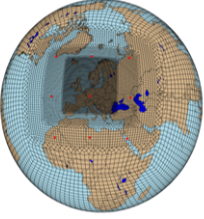
\includegraphics[height=4.5cm]{images/gg-a.png}
  \caption{Selected domains from our use cases. From left to right: interactive
    analysis of sea bass fish track reconstructions on biologging tag data (sea bass)
    with low resolution marine physics data; electron
    density of benzene molecule computed with Octopus; NorESM artic grid for running Earth System Modelling experiments.
    (Background map: \copyright
    OpenStreetMap contributors ) \label{fig:applications}}
  \TODO{Add at least one more.}
\end{figure}

\subsubsection{Open Source ecosystem}\label{sec:opensource}\TODO{Should the
  title be a bit more specific for Binder /Jupyter?}


The Binder Project \cite{binder} (\url{https://jupyter.org/binder}) is
a subproject of the Jupyter project, although it is not confined to be
useful only for notebooks.
\emph{Project Jupyter} \cite{Jupyter}, which has grown increasingly popular in the scientific
computing community, has become the \emph{lingua franca} of interactive
computing in both academia and industry \cite{Perkel2018}. The main goal of Project Jupyter
is to provide a consistent set of tools to improve researchers'
workflows from the exploratory phase of the analysis to the communication
of the results \cite{Kluyver2016,Granger2021}.

\TODO{Lost "what is Jupyter" in reshuffle}

The key components of the Binder software are \repotodocker{}
(Section~\ref{sec:repo2docker}) and \binderhub{}~\ref{sec:binderhub}. The \repotodocker{} tool
creates a software environment inside a Docker container from a software
specification in a repository. \binderhub{} starts a Jupyter notebook server
within this container from which the user can execute the notebooks from the
repository.

\emph{\mybinder{}} (see \ref{sec:mybinder}) is a service provided by the \myemph{BinderHub
Federation} that collectively host a service running the Binder software
under the URL \url{https://mybinder.org}. (This is the service we made use of in the example
of section~\ref{sec:reproducibility-example}.)

The BinderHub Federation is currently composed of three deployments of the BinderHub software

\begin{itemize}
\item \url{https://gke.mybinder.org}, operated by the Binder team, and hosted on Google Cloud,
\item \url{https://ovh.mybinder.org}, operated and hosted by OVH,
\item \url{https://gesis.mybinder.org}, operated and hosted by GESIS.
\end{itemize}

The focus for this proposal is to improve \repotodocker{}. In particular,
\repotodocker{} solves the software environment challenge (see
Section~\ref{sec:reproducibility-challenges}) in a generic way and is independent
from Jupyter notebooks.


\paragraph{Binder example}
\label{binder-how-does-it-work}

\mbox{}\\

The currently most common reproducibility use case -- with the current state of the
\textbf{Binder tools} -- is the one we introduced in
Section~\ref{sec:reproducibility-example} using the \mybinder{} service. We will use this to
describe the role of the individual components of the Binder tools:

\begin{figure}[ht]
  \centering
    \includegraphics[width=0.7\textwidth]{images/mybinder.png}
    \caption{Home page of the \mybinder{} service.}
    \label{fig:mybinder-homepage}
\end{figure}

\begin{compactitem}
\item The \binderhub{} service is given a URL that encodes the location of the data
  repository\footnote{For example the
    {\url{https://mybinder.org/v2/gh/fangohr/reproducibility-repository-example/HEAD?labpath=figure1.ipynb}}
    refers to the GitHub repository ``reproducibility-repository-example'' of the
    github user ``fangohr'', asking to open the ``figure1.ipynb'' file.}
  (see Figure~\ref{fig:mybinder-homepage})
\item \binderhub{} will use
  \repotodocker{} to create a \textbf{software environment} (Docker image)
  in which the notebooks or scripts from the repository can be executed.
\item \repotodocker{} searches the repository for \textbf{software specifications}.
\item \repotodocker{} constructs the \textbf{software environment}
  from the \textbf{software specification(s)} (a Docker image).
\item \binderhub{} asks \JupyterHub to start
  a \textbf{notebook session} in this \textbf{software environment}.
\item \binderhub{} forwards the user who requested this environment to
  the URL at which the repository (or a particular notebook) can be explored
  from within the Jupyter application.
\end{compactitem}


\paragraph{\repotodocker}\label{sec:repo2docker}
The \repotodocker{} tool aims to \myemph{automate existing practices} for reproducible environment specification.
It finds \emph{standard} environment specifications and produces \emph{typical} installation commands,
constructing an environment in a Docker container image.
\repotodocker{} can fetch a remote repository and build a software
environment for this repository. Currently, \repotodocker{} can retrieve
repositories from the following services and formats: GitHub, Gist, Git, GitLab,
Zenodo, Hydroshare, Figshare, and Dataverse.

For the automatic building of reproducible computational environments,
\repotodocker{} understands commonly used conventions for environment specifications and
community standard tools such as Docker, conda, mamba, and pip.
\repotodocker{} is successful enough to be widely adopted,
but many shortcomings have been identified,
especially when a repository contains an \emph{incomplete} specification.
A common issue is to produce an environment that works when published,
but which may produce a non-working environment at a later point in time,
due to version drift and insufficiently strict specifications.
Additionally, community practices not yet supported by \repotodocker{} have been proposed by their respective community members,
but the \repotodocker{} team has not had the funding support to incorporate and maintain them.

\paragraph{BinderHub}\label{sec:binderhub}
BinderHub is software for hosting a web service built on \repotodocker{} and
JupyterHub where individuals can share reproducible environments for
immediate and free interaction by readers in their browser.

The BinderHub software exposes \repotodocker{} and Jupyter as a service,
allowing one-click reproduction of published environments for \emph{interactive exploration}.
BinderHub is shown to work well,
but has limited application due to technical limitations,
such as its reliance on the Kubernetes deployment platform,
or challenges with combining the convenience of BinderHub's anonymous-by-default model
with authenticated and/or performant access to large data or compute resources.

While the \repotodocker{} terminal utility \emph{can} technically be deployed anywhere,
the technical expertise required is dramatically greater than a single click on a website such as mybinder.org.

\paragraph{The \mybinder{} service}\label{sec:mybinder}

% \mbox{}\\

The \mybinder{} service is run by the \emph{BinderHub
Federation}\footnote{\url{https://mybinder.readthedocs.io/en/latest/about/federation.html}}
of organisations. Collectively, they host a service running the BinderHub software
which can be reached from \url{https://mybinder.org}.

The service is actively used with approximately 200,000 sessions being
requested and delivered by the \mybinder{} service every week in 2021. The number
of sessions is growing from approximately 10,000 per day in November 2018
(beginning of the available records) to about 30,000 per day in 2022. We have
identified 60,000 unique repositories published in the last few years which have
used the \mybinder{} service. The data is available~\cite{mybinder-archive}.

Examples of reproducible repositories that make use of the \mybinder service
include reproducible research repositories
\cite{GitHubRepoExampleAlbert2016,Beg2021}, interactive textbooks
\cite{Fangohr2022,Zeller2022} and citizen science and outreach activities
\cite{ligo-open-science,OSCOVIDA2022}.

This \TheProject{} project will not provide or operate a BinderHub service (such as the global
``\url{https://mybinder.org}'' instance). The resulting improvements, however, will be
immediately available to all operators of BinderHubs, including \mybinder{}.


\TODO{Add info on links we have with our own providers and what role they play in the project e.g.
deployment of binder services with newly developed features}

\subsubsection{Technical Readiness Level (TRL)}

TRL is unusual for Binder tools, because they are tools that can be used in many ways,
and they can be described as having a different TRL \emph{in different contexts}.

The Binder software and service demonstration at mybinder.org is TRL 6,
where scope \emph{excludes} long-term robustness.
The Binder software for deploying services with authenticated access to data is TRL 3.
We will bring it to TRL 6.
The Binder tool repo2docker when targeting robust reproducible environments is TRL 4.
We will bring it to TRL 6.



\subsubsection{Community Engagement Panel}\label{sec:community-engagement-panel}
The Community Engagement Panel (CEP) is a forum to bring together
  representatives of current and potential user communities of Binder tools.
  Through the community engagement panel we want to maximise the interaction between existing and new users.
  This will help shape the software features so that we can
  achieve the highest possible impact for reproducibility in science.

  Stakeholders for the topic of reproducibility that should be represented in the
  community engagement panel include researchers, research infrastructure
  providers, publishers, research councils, librarians, and educators.

  We have already secured agreement from the following to be part of the panel,
and will extend this if funded:
\begin{itemize}
\item Suzanne Dumouchel, Head of European Cooperation at TGIR Huma-Num CNRS unit, a large infrastructure for
digital humanities and member of the EOSC Association Board of Directors. She is the partnerships coordinator
of OPERAS Research Infrastructure, devoted to scholarly communication in Social Sciences and Humanities and is a member of DARIAH ERIC Coordination Office,
dedicated to Digital Arts and Humanities. She is also the scientific coordinator of TRIPLE, H2020 project
(INFRAEOSC2). Strongly committed to the Open Science movement and to the promotion of research in Social Sciences
and Humanities (SSH), she is particularly active in the field of research infrastructures.
\item Andy Götz, Software Group Leader at European Radiation Synchrotron
  Facility (ESRF), coordinator of the EOSC project PaNOSC for making data from
  photon and neutron facilities FAIR, and chairman of the IT working Group of
  the ``League of European Accelerator-based Photon Sources'' (LEAPS). The LEAPS
  facilities wish to enable their users to create reproducible publications
  based on large data sets captured at the light sources.
\item Paula Andrea Martinez, Project Coordinator - Software Program, \href{https://ardc.edu.au/}{Australian Research Data Commons} (ARDC).
She is also the co-chair of the \href{https://www.rd-alliance.org/groups/fair-research-software-fair4rs-wg}{FAIR4RS RDA Working Group} and
Community Manager at \href{https://www.researchsoft.org/}{Research Software Alliance} (ReSA), and actively contributing
to increase the visibility of research software.
\item Aleksandra Nenadic, Training Lead of the Software Sustainability Institute,
based at the University of Manchester (UK). She is also an active member and
promoter of the Carpentries community and involved as an instructor,
instructor trainer, mentor, workshop organiser and regional coordinator
for the UK, driving and supporting new material creation using the
Carpentries collaborative and pedagogical lesson development principles.
\item Gergely Sipos, head of services, solutions and support department at the
  EGI Foundation. He is representing EGI, ``Advanced Computing for EOSC''
  (EGI-ACE) and the EOSC Compute Platform, which are working on a large-scale
  deployment of BinderHub as part of their services for researchers in Europe
  and beyond.
\item Violaine Louvet, head of GRICAD (Grenoble Alpe Research -
 Scientific Computing and Data Infrastructure), supported by
 CNRS, Grenoble Alpes University and INRIA. GRICAD is a Tier 2
 infrastructure and provides data and computing resources to all the
 science communities in Grenoble. In particular, GRICAD provides HPC,
 HTC, cloud and storage resources for all the disciplinary fields,
 from computer sciences to human sciences and health. GRICAD
 also offers a JupyterHub and a BinderHub platform. We are also very
 involved in helping the scientific communities and in training activities.
 \item Rollin Thomas, Big Data Architect at HPC expert at the National Energy
  Research Scientific Computing Center at Lawrence Berkeley National Laboratory
  (US). He represents the HPC community, and focuses on interactivity,
  real-time, and reproducibility in supercomputing for science.
\item Andreas Zeller, Professor of Software Engineering at Saarland University. He uses Notebooks
  to provide open-source text books to his students and the world-wide
  community of readers. He will represent Binder users in academia, who use it
  to deliver zero-install computational environments for educational
  purposes.
\end{itemize}


\subsubsection{Gender aspects}\label{sec:gender}

\eucommentary{Describe how the gender dimension (i.e. sex and/or gender
  analysis) is taken into account in the project's research and innovation
  content [e.g. 1 page]. If you do not consider such a gender dimension to be
  relevant in your project, please provide a justification.}

\eucommentary{
	Note: This section is mandatory except for topics which have been identified
  in the work programme as not requiring the integration of the gender dimension
  into R\&I content.
}

\eucommentary{
	Remember that that this question relates to the content of the planned
  research and innovation activities, and not to gender balance in the teams in
  charge of carrying out the project.
}

\eucommentary{
	Sex and gender analysis refers to biological characteristics and
  social/cultural factors respectively. For guidance on methods of sex/gender
  analysis and the issues to be taken into account, please refer to
  \url{https://ec.europa.eu/info/news/gendered-innovations-2-2020-nov-24\_en}
}

In order to address gender issues, \TheProject is committed to implement
communication and outreach activities for promoting the role of women and underrepresented groups in science
and STEM: i) present showcases to demonstrate the results of the project through
the eyes of female Research Software Engineers and researchers; ii)
systematically offer hybrid or online training opportunities to encompass the
lack of mobility of some potential attendees; iii) monitor gender participation
to our training, workshops, and hackathons and track progress. Members of the
consortium are involved in a number of programmes and activities who aim at
upskilling women and diversity and inclusion, for instance The Carpentries and
CodeRefinery training programmes and mentoring programs such as Outreachy or
Open Life Science.

\subsubsection{National and international research or innovation activities}

\eucommentary{Describe any national or international research and innovation
  activities whose results will feed into the project, and how that link will be
  established; [e.g. 1 pages]}
\TOWRITE{}{}

The SOURCE project, as part of the overall Jupyter environment, will intrinsically build on the achievements of many
 national and European and international research and innovative developments, which have been produced or are 
 being implemented in research projects in which research infrastructures and project partners are or have been 
 involved.

The science applications build on the outcomes of National, Nordic, European and/or international research and 
innovation projects and initiatives. Both Ifremer and the University of Oslo are active members of the international 
Pangeo\footnote{https://pangeo.io/} Big data Geosciences Community.

Ifremer, through its co-ownership of Mercator Ocean International\footnote{https://www.mercator-ocean.eu/},
 participate in the operation of the Copernicus Marine Environment Monitoring Service (CMEMS), 
 a part of Copernicus, the European Union’s Earth Observation Programme and is also actively involved in the 
 development of a Digital Twin of the Ocean that will be fully compatible with the Destination Earth (DestinE\footnote{https://digital-strategy.ec.europa.eu/en/policies/destination-earth})
 architecture and supports the European's Digital Strategy and Green Deal Package.   

\subsubsection{Interdisciplinarity}

\eucommentary{Explain how expertise and methods from different disciplines will be brought together and integrated in pursuit of your objectives. If you consider that an inter-disciplinary approach is unnecessary in the context of the proposed work, please provide a justification. [e.g. 1/2 page]
}
\TheProject{} brings together research software engineers with researchers from
multiple science domains to develop tools and methods that work across
scientific domains. An interdisciplinary approach is key to our success
(see Section~\ref{sec:complementarity-and-interdisciplinarity}).

\subsubsection{Open science practices and implementation}\label{sec:open-science-practices}

\TheProject will make use of open source licensed software, packages and libraries, following the \href{https://opensource.org/licenses}{OSI recommendations}.

All codes in this project will be Open Source and collaboratively developed using GitHub, following best software engineering practice
such as version control, tests and continuous integration.
Training materials will be collaboratively developed through the \href{https://carpentries-incubator.org/}{Carpentries Incubator}
using the \href{https://cdh.carpentries.org/}{Carpentries Curriculum Development Handbook}: all Carpentries lessons are licensed under
the \href{https://creativecommons.org/licenses/by/4.0/legalcode}{Creative Commons Attribution version 4.0 (CC-BY)} and any related software under
the \href{https://opensource.org/licenses/MIT}{MIT license}.

Use cases and showcases will only make use of data that are openly available.

All publications and/or any research data produced within \TheProject will be published Open Access.


\eucommentary{Describe how appropriate open science practices are implemented as
   an integral part of the proposed methodology. Show how the choice of practices
   and their implementation are adapted to the nature of your work, in a way that
   will increase the chances of the project delivering on its objectives [e.g. 1
   page].
%
   If you believe that none of these practices are appropriate for your
   project, please provide a justification here.
   }

\eucommentary{Open science is an approach based on open cooperative work and systematic
   sharing of knowledge and tools as early and widely as possible in the process.
   Open science practices include early and open sharing of research (for example
   through preregistration, registered reports, pre-prints, or crowd-sourcing);
   research output management; measures to ensure reproducibility of research
   outputs; providing open access to research outputs (such as publications,
   data, software, models, algorithms, and workflows); participation in open
   peer-review; and involving all relevant knowledge actors including citizens,
   civil society and end users in the co-creation of R\&I agendas and contents
   (such as citizen science).}

\eucommentary{Please note that this question does not refer to outreach actions that may be
   planned as part of communication, dissemination and exploitation activities.
These aspects should instead be described below under 'Impact'.}

\TOWRITE{}{}

\subsubsection{Research Data Management and management of other outputs}

The Data Management Plan (DMP) will be prepared and regularly updated within WP1.

Except for the software and usage data described below,
\TheProject activities will not generate or collect data.
While we have many demonstrators that interact with data, they do not generate or collect that
data themselves, but rather provide analytical mechanisms or access to data governed by
existing data management plans and data policies of project partners at each site,
as well as publicly accessible open data.

All data generated, collected, processed and stored will be made available following the
relevant standards and regulations. Processing of personal data in relation to training,
hackathons and/or workshop events will comply with GDPR regulations e.g. data
anonymization and minimization before sharing.
Procedures to monitor the real-time effectiveness of our dissemination and
communication strategies will also be GDPR compliant.
We have no plans to collect or produce personally identifiable information (PII)
during the project.

\noindent \textbf{Software} \\
Most research data from \TheProject will take the form of code.
All code produced by \TheProject will be developed in the public using open
source licenses (see Section~\ref{sec:open-science-practices}).
Milestone achievements of the software may be archived
in separate repositories such as Zenodo,
e.g. to coincide with publications.

\noindent \textbf{Service usage data} \\
Any data collected through the operation of public services
(e.g. popularity data for public open science repositories)
will be fully anonymised to the satisfaction of relevant best privacy practices and regulations, such as GDPR,
and made publicly available in the standard JSON Lines format,
as is done already for mybinder.org \cite{mybinder-archive}.
This is very small data and easily archived on free hosting services such as GitHub,
and will be made available under the Creative-Commons Universal Public Domain Dedication (CC0).
There is no cost to the project associated with archiving this data long-term.


\eucommentary{
Research data management and management of other research outputs: Applicants
generating/collecting data and/or other research outputs (except for
publications) during the project must provide maximum 1 page on how the data/
research outputs will be managed in line with the FAIR principles (Findable,
Accessible, Interoperable, Reusable), addressing the following (the description
should be specific to your project): [1 page]
}

\eucommentary{
Types of data/research outputs (e.g. experimental, observational, images, text,
numerical) and their estimated size; if applicable, combination with, and
provenance of, existing data.
}

\eucommentary{
Findability of data/research outputs: Types of persistent and uniqueidentifiers
(e.g. digital object identifiers) and trusted repositories that will be used.
}

\eucommentary{
Accessibility of data/research outputs: IPR considerations and timeline for open
access (if open access not provided, explain why); provisions for access to
restricted data for verification purposes.
}

\eucommentary{
Interoperability of data/research outputs: Standards, formats and vocabularies
for data and metadata. Reusability of data/research outputs:  Licenses for data
sharing and re-use (e.g. Creative Commons, Open Data Commons); availability of
tools/software/models for data generation. }

\TOWRITE{}{}

\begin{draft}
\section*{Todo list for missing subsections}
\begin{verbatim}
- [ ] 1 page: National or international research or innovation activities
- [ ] 0.5 page: bringing together expertise and methods from different disciplines
- [ ] 0.5 page: social science and humanities - how do we integrate them, or why do we not need them
- [X] 1 page: gender dimension.
- [ ] 1 page: open science practices and implementation
- [ ] 1 page: research data management and management of other research outputs. (Also FAIR)
\end{verbatim}
\end{draft}

%%% Local Variables:
%%% mode: latex
%%% TeX-master: "proposal"
%%% End:
